\documentclass[a4paper, 11pt]{article}
\usepackage{kotex}
\usepackage{amsmath, amssymb, amsthm}
\usepackage{graphicx}
\usepackage{enumitem}

\title{향후 인기 게임 트렌드 예상: 인기 게임 분석으로}
\author{202255663 설종환}
\date{}
\begin{document}

\maketitle

\section{서론}
게임 산업은 지속적으로 변화하고 발전해 왔으며, 2020년 이후 COVID-19 팬데믹의 영향으로 새로운 게임 트렌드가 형성되어왔다. 사회적 거리두기와 봉쇄 조치로 사람들이 집에서 보내는 시간이 증가하면서, 게임은 더 이상 단순한 여가 활동을 넘어서 사회적 상호작용의 중요한 수단이 되었다. 이렇듯 게임이 우리 삶에 끼치는 영향이 증가함에 따라, 본 보고서에서는 2020년부터 2022년까지의 인기 게임들과 역대 가장 많이 팔린 게임에 대한 분석을 토대로 향후 인기 게임 트렌드가 어떻게 형성될 것인지 예측해보고자 한다.

\section{본론}

\subsection{2020년 상위 매출 10위 게임들 분석}
2020년은 사람들과 소통 및 상호작용이 활발한 소셜 기능과 커뮤니티 기반 플레이가 강화된 형태의 게임들이 많은 인기를 끌었다. COVID-19 팬데믹으로 인해 많은 사람들이 집에서 시간을 보내며 게임을 주요 엔터테인먼트로 삼았던 것이 그 요인으로 보이며, 덕분에 게임 시장의 매출과 사용자 수가 폭발적으로 증가했다. 이에 따라, 2020년 글로벌 게임 시장 매출 상위 게임들도 대부분 온라인 멀티플레이어 게임이다.

\begin{table}[h!]
    \resizebox{\textwidth}{!}{%
    \begin{tabular}{|ccccc|}
    \hline
    \textbf{매출 순위} & \textbf{게임} & \textbf{장르} & \textbf{플랫폼} & \textbf{매출액(달러)} \\ \hline
    1 & PUBG(배틀 그라운드) & 배틀 로얄 & PC, 콘솔, 모바일, 클라우드 & \$28.2억 \\
    2 & Honor of Kings (펜타스톰) & MOBA & 모바일, 닌텐도 & \$25.6억 \\
    3 & Roblox & MMO & PC, 콘솔, 모바일, VR & \$23억 \\ \hline
    4 & Garena Free Fire & 배틀 로얄 & 모바일 & \$21.3억 \\
    5 & Animal Crossing: New Horizons & 소셜 시뮬레이션 & 닌텐도 스위치 & \$20억 \\
    6 & Pokémon Go & AR(증강 현실) & 모바일 & \$19.2억 \\ \hline
    7 & Call of Duty: Modern Warfare / Warzone & FPS / 배틀 로얄 & PC, 콘솔 & \$19.1억 \\
    8 & League of Legends & MOBA & PC & \$17.5억 \\
    9 & Candy Crush Saga & 퍼즐 & 모바일 & \$16.6억 \\
    10 & AFK Arena & RPG & 모바일 & \$14.5억 \\ \hline
    \end{tabular}%
    }
    \caption{2020년 상위 매출 10위 게임 \cite{2020top10}}
\end{table}

2020년의 게임 트렌드는 COVID-19 팬데믹의 이례적인 상황에 지대한 영향을 받았으며, 타인과의 교류 및 소통과 같은 인간의 기본 욕구에 영향을 끼칠 수 있는 요인이 게임 트렌드를 좌우할 수도 있다는 것을 살펴볼 수 있었다. 사회적 거리두기와 같은 제한 조치로 인해, 사람들은 타인과의 소통과 교류에 대한 욕구가 더욱 커졌고, 그 결과 온라인 멀티플레이 기능과 소셜 요소를 포함한 게임들이 크게 인기를 끌었다. 또한 상위 10위 게임들 중 7개의 게임이 모바일 플랫폼을 포함한다는 점에서, 언제 어디서나 쉽게 즐길 수 있는 게임이 인기를 끌고 있음을 확인할 수 있다.

\subsection{2021년 상위 매출 10위 게임들 분석}
2021년에는 RPG 게임이 신흥 강자로 떠오르며, 모바일 플랫폼 게임과 배틀 로얄 장르가 2020년에 이어 여전히 인기를 이어갔다. 던전앤파이터는 중국 시장에서 큰 성공을 거두었으며, 원신은 모바일 오픈월드 RPG라는 독특한 경험을 제공하며 큰 인기를 끌었다. 또한, 2020년 매출 1위와 2위를 차지했던 배틀그라운드와 펜타스톰의 매출은 각각 약 14\% 증가하며 그 인기를 더욱 공고히 했다.

\begin{table}[h!]
    \resizebox{\textwidth}{!}{%
    \begin{tabular}{|ccccc|}
    \hline
    \textbf{매출 순위} & \textbf{게임} & \textbf{장르} & \textbf{플랫폼} & \textbf{매출액(달러)} \\ \hline
    1 & PUBG(배틀 그라운드) & 배틀 로얄 & PC, 콘솔, 모바일, 클라우드 & \$32.33억 \\
    2 & Honor of Kings (펜타스톰) & MOBA & 모바일, 닌텐도 스위치 & \$28억 \\
    3 & Dungeon \& Fighter Online (DFO) & RPG & PC & \$27억 \\ \hline
    4 & Genshin Impact & 오픈월드 RPG & PC, 콘솔, 모바일 & \$19억 \\
    5 & Roblox & MMO & PC, 콘솔, 모바일, VR & \$14억 \\
    6 & Coin Master & 캐주얼 & 모바일 & \$14억 \\ \hline
    7 & Pokémon Go & AR(증강 현실) & 모바일 & \$13억 \\
    8 & Candy Crush Saga & 퍼즐 & 모바일 & \$13억 \\
    9 & Garena Free Fire & 배틀 로얄 & 모바일 & \$12억 \\
    10 & League of Legends & MOBA & PC & \$11억 \\ \hline
    \end{tabular}%
    }
    \caption{2021년 상위 매출 10위 게임 \cite{2021top10}}
\end{table}

2021년도는 COVID-19의 지속적인 영향을 받아 2020년과 유사한 양상을 보였다. 그러나 그 중에서도 모바일 오픈월드 RPG 장르의 전례 없는 대성공과 모바일 플랫폼의 지속적인 강세가 특히 두드러진다. 배틀그라운드의 대흥행이 배틀 로얄 장르의 유행을 선도했듯, 원신의 성공 또한 비슷한 흐름을 이끌어낼 가능성이 있다.

2020년에는 7개의 게임이 모바일 플랫폼을 지원했으며, 2021년에는 그 비중이 8개로 증가했다. 특히 주목할 점은 같은 장르인 펜타스톰과 리그 오브 레전드의 매출 변화이다. 모바일 게임인 펜타스톰은 1년 전과 비교해 매출이 증가한 반면, PC게임인 리그 오브 레전드는 매출이 감소하였다. 이는 언제 어디서나, 그리고 누워서 편안하게 즐길 수 있는 모바일 게임이 그 강세를 지속적으로 이어나갈 수 있음을 시사한다.

\subsection{2022년 상위 매출 10위 게임들 분석}
2022년은 전체적으로 게임 시장 매출이 소폭 감소했으며, PC와 콘솔 플랫폼, 그리고 RPG 장르의 인기가 두드러진 해였다. COVID-19로 인한 게임 산업의 호황이 일상의 회복과 함께 서서히 정상화되면서, 게임에 대한 수요도 자연스럽게 줄어든 것으로 보인다.\cite{ITSGame}엘든 링과 콜 오브 듀티의 성공은 콘솔 게임의 인기를 다시 한 번 증명했으며, 상위 10위 게임 중 5개가 RPG 장르로, RPG의 강세가 뚜렷하게 나타났다. 또한, 펜타스톰, 배틀그라운드, 던전앤파이터, 원신은 2021년에 이어 매출 상위권을 유지하며 그 인기를 지속했다.

\begin{table}[h!]
    \resizebox{\textwidth}{!}{%
    \begin{tabular}{|ccccc|}
    \hline
    \textbf{매출 순위} & \textbf{게임} & \textbf{장르} & \textbf{플랫폼} & \textbf{매출액(달러)} \\ \hline
    1 & Honor of Kings (펜타스톰) & MOBA & 모바일, 닌텐도 스위치 & \$28억 \\
    2 & PUBG(배틀 그라운드) & 배틀 로얄 & PC, 콘솔, 모바일, 클라우드 & \$25.5억 \\
    3 & Dungeon \& Fighter Online (DFO) & RPG & PC & \$20억 \\ \hline
    4 & Genshin Impact & 오픈월드 RPG & PC, 콘솔, 모바일 & \$19억 \\
    5 & Candy Crush Saga & 퍼즐 & PC, 모바일 & \$13억 \\
    6 & Pokémon Scarlet/Violet & RPG & 닌텐도 스위치 & \$12.4억 \\ \hline
    7 & Lineage & MMORPG & PC & \$12.35억 \\
    8 & Elden Ring & 오픈월드 RPG & PC, 콘솔 & \$12억 \\
    9 & Roblox & MMO & PC, 모바일, 콘솔, VR & \$11억 \\
    10 & Call of Duty: Modern Warfare II & FPS & PC, 콘솔 & \$10억 \\ \hline
    \end{tabular}%
    }
    \caption{2022년 상위 매출 10위 게임 \cite{2022top10}}
\end{table}

엘든 링과 콜 오브 듀티와 같은 PC, 콘솔 플랫폼 게임의 성공이 주목할 만하며, 모바일 플랫폼 게임의 비중이 2021년 8개에서 2022년에 5개로 줄었다. 이는 모바일 게임의 인기가 감소했다는 의미는 아니다. 2022년에 전체적인 게임 시장 매출이 감소했음에도, 모바일 게임은 매출은 변동이 없었기 때문이다(펜타스톰 \$28억\(\rightarrow\)\$28억, 캔디 크러시 사가 \$13억\(\rightarrow\)\$13억).

PC와 콘솔 플랫폼에서의 좋은 그래픽과 풍부한 조작감을 통한 혁신적이고 몰입감 높은 게임들이 좋은 성과를 거두었다. 이를 통해 풍성한 게임 경험을 제공할 수 있는 플랫폼의 중요성이 다시 부각되었다. 따라서 COVID-19 이후 멀티플레이어와 모바일 중심의 트렌드에서 벗어나, 엘든 링과 원신처럼 싱글 플레이어 중심의 오픈월드 게임같이 다양한 플랫폼과 장르의 게임들이 흥행할 수 있다는 점이 입증되며 새로운 트렌드의 가능성을 열었다. 결론적으로 모바일 게임의 강세는 여전히 유지되고 있지만, PC와 콘솔 플랫폼의 오픈월드 RPG 및 배틀 로얄 장르가 강력한 입지를 확보하고 있다.

\subsection{역대 판매량 상위 10위 게임들 분석}
사람들이 앞으로 어떤 게임을 즐겨할지를 예측하기 전에, 이때까지 어떤 게임에 열광해 왔는지 알아보려 한다. 역대 게임 판매량 상위권을 차지한 게임들은 주로 다양한 플랫폼에서 출시된, 긴 시간 동안 꾸준히 사랑받아온 게임들이 많다. 이러한 게임들이 오랜 시간 동안 인기를 유지할 수 있었던 이유는 단순한 게임 플레이 이상의 가치를 제공했기 때문이다. 따라서 아래 표의 게임들에 대한 분석은 향후 게임 트렌드를 예측하는 데 단서를 제공해줄 수 있다.

\begin{table}[h!]
    \resizebox{\textwidth}{!}{%
    \begin{tabular}{|ccccc|}
    \hline
    \textbf{판매 순위} & \textbf{게임} & \textbf{장르} & \textbf{플랫폼} & \textbf{판매량(장)} \\ \hline
    1 & Minecraft & 샌드박스 & PC & 3억 \\
    2 & GTA5 & 오픈월드 액션 어드벤처 & PC, 콘솔 & 1.95억 \\
    3 & Tetris & 퍼즐 & PC, 모바일 & 1억 \\ \hline
    4 & Wii Sports & 스포츠 & Wii & 8300만 \\
    5 & PUBG: Battlegrounds & 배틀 로얄 & PC, 콘솔 & 7500만 \\
    6 & Mario Kart 8 Deluxe & 레이싱 & 닌텐도 스위치 & 6900만 \\ \hline
    7 & Red Dead Redemption 2 & 오픈월드 액션 어드벤처 & PC, 콘솔 & 6100만 \\
    8 & Super Mario Bros & 플랫포머 & NES & 5800만 \\
    9 & Overwatch & FPS & PC, 콘솔 & 5000만 \\
    10 & The Witcher 3: Wild Hunt & 오픈월드 액션 RPG & PC, 콘솔 & 5000만 \\ \hline
    \end{tabular}%
    }
    \caption{역대 판매량 상위 10위 게임 \cite{alltimetop10}}
\end{table}

위 게임들은 각기 다른 장르에서 선구자적인 역할을 하거나 해당 장르의 재미를 극대화하는데 정점을 찍었다는 특징을 가지고 있다. 마인크래프트, 테트리스, 배틀그라운드는, 슈퍼마리오 등은 그들 장르에서 혁신적이고 깊은 경험을 제공하며 큰 인기를 끌었으며 그 장르의 유행을 선도한 대표 게임이 되었다. 

GTA5, 레드 데드 리뎀션 2, 위쳐 3와 같은 오픈월드 장르의 게임들이 유일하게 역대 판매량 상위 10위에 3개나 포함된 것은, 플레이어들이 게임을 통해 현실에서 하지 못하는 일을 경험하면서 자유를 느끼고, 이러한 경험에서 큰 재미를 얻는다는 것을 시사한다. 오픈월드 게임은 플레이어에게 높은 자유도를 제공하여 스스로 목표를 설정하고 다양한 방식으로 문제를 해결할 수 있는 기회를 주기 때문에, 이 장르의 매력은 앞으로도 지속될 가능성이 크다. 따라서 이러한 게임들의 성공은 플레이어들이 다양한 장르에서 자유로운 선택과 창의적인 경험을 원하는 경향을 반영하며, 앞으로의 게임 산업에서도 비슷한 흐름이 지속될 것으로 예상된다.

\subsection{인기 게임들 분석 정리}
\begin{enumerate}[label=\arabic*.]
    \item \textbf{모바일 게임의 지속적 강세} \\
    2020년과 2021년 동안 모바일 게임이 게임 매출 상위권을 점령하면서 강력한 입지를 다졌다. 2022년에도 이러한 흐름이 이어졌으며, \textit{펜타스톰}, \textit{캔디 크러시 사가}, \textit{포켓몬 고} 등의 게임은 지속적인 매출을 기록했다.

    이러한 성공은 모바일 게임의 휴대성과 접근성 덕분에 이루어진 것으로 분석된다. 스마트폰 보급률이 높아짐에 따라 누구나 쉽게 접근할 수 있는 모바일 게임은 시간과 장소에 구애받지 않고 즐길 수 있다는 장점을 제공한다. 이러한 요소들은 모바일 게임이 앞으로도 게임 산업의 중요한 축으로 자리 잡을 것임을 시사한다. 특히, \textit{원신}과 같은 모바일 오픈월드 RPG의 성공은 복잡한 게임 조작과 경험을 요구하는 장르조차도 모바일 플랫폼에서 성공할 수 있음을 보여준다.

    \item \textbf{오픈월드 게임의 시대불문 인기} \\
    오픈월드 게임은 여러 해 동안 꾸준히 인기를 끌어온 장르다. 역대 판매량 상위 10위 게임 중 3개의 게임 (\textit{GTA 5}, \textit{레드 데드 리뎀션 2}, \textit{위쳐 3})이 오픈월드 게임으로, 이 장르가 제공하는 높은 자유도와 탐험의 재미는 게이머들에게 지속적인 인기를 얻고 있으며 2022년의 \textit{엘든 링}의 성공 역시 이러한 흐름을 보여준다. AI와 같은 게임 기술의 발전과 더불어 더욱 넓고 세밀한 오픈월드 환경이 제공되면서, 이 장르는 향후 더욱 발전할 것으로 기대된다.

    \item \textbf{PC와 콘솔 플랫폼의 부상과 RPG 장르의 인기} \\
    2022년의 매출 상위권 게임들은 PC와 콘솔 플랫폼 게임의 강세를 보여준다. 이는 COVID-19 팬데믹이 끝난 후 일상으로의 복귀와 함께 사람들이 모바일 게임에서 PC와 콘솔 게임으로 눈을 돌리기 시작한 흐름으로 해석된다. 특히, \textit{엘든 링}, \textit{원신} 등의 오픈월드 RPG 게임들은 플레이어에게 몰입도 높은 경험과 깊은 스토리라인을 제공하며, 강력한 팬층을 형성했다. RPG 장르는 캐릭터 성장과 퀘스트를 통한 긴 시간의 게임 플레이를 가능하게 하여, 앞으로도 다양한 플랫폼에서 주목받을 가능성이 크다.

    \item \textbf{차별화된 방식을 통한 혁신적 경험의 인기} \\
    2020년대 초반의 성공적인 게임들 중에서, 그들 장르 속에서 기존의 틀을 벗어나 새로운 방식으로 게임을 재구성하여 혁신적인 경험을 제공한 게임들이 있다.
    
    \textit{포켓몬 고}는 당시 최신기술인 AR을 스마트폰 카메라와 GPS 기술을 결합해 이전에 경험하지 못한 현실 세계와 게임을 연결하는 재미를 선사했다. \textit{원신}은 이전까지 간단한 퍼즐이나 턴제 RPG처럼 캐주얼한 장르가 주를 이룬 모바일 게임에서, 오픈월드 RPG라는 장르를 효과적으로 선보이며 모바일 게임에서의 혁신적인 경험을 제공했다. \textit{엘든 링}은 기존 소울라이크 게임들처럼 제한된 공간에서의 전투와 스토리 진행을 벗어나, 자유롭게 탐험할 수 있는 방대한 세계를 제공하며 새로운 방식의 몰입을 선사했다. 
    
    이처럼 혁신적인 접근은 단순히 장르의 변화가 아닌, 기술적 발전과 창의적인 게임 설계가 결합되어 새로운 게임 경험을 창출하는 데 중요한 역할을 한다. 또한 새로운 기술이 계속해서 개발되고 있는 현 시점에 있어, 이러한 트랜드는 중요한 요소로 자리 잡을 가능성이 크다.
\end{enumerate}

\section{결론}
이 분석을 바탕으로, 향후 게임 트렌드에서 중요한 요소는 모바일 플랫폼의 지속적인 강세, 오픈월드 게임의 인기, PC와 콘솔 플랫폼에서의 RPG 장르의 부상, 그리고 차별화된 방식을 통한 혁신적 경험의 인기이다. 특히 2020년부터 2022년까지의 장르별 매출 변화에서 RPG 장르의 매출이 증가한 점은 주목할 만하다.

\begin{figure}[h!]
    \centering
    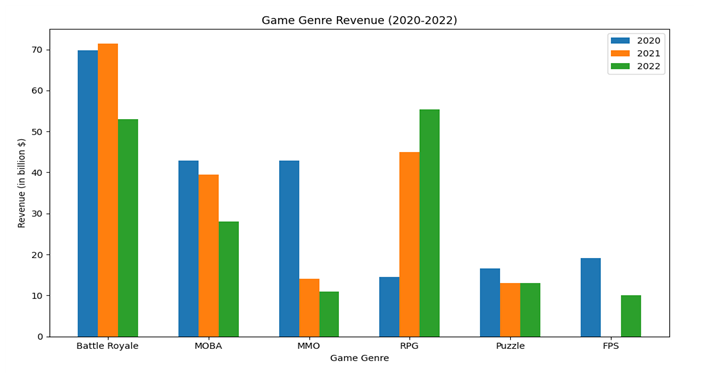
\includegraphics[width=\textwidth]{resource/sales_change__graph.png}
    \caption{2020-2022 장르별 매출 변화(표1,2,3에 근거)}
    \label{sales change according to game genre from 2020 to 2022}
\end{figure}

따라서 RPG 장르는 앞으로도 다양한 플랫폼에서 인기를 끌 것으로 예상된다. 플레이어들이 더욱 풍부하고 혁신적인 경험을 느끼는데 있어 RPG 장르, 특히 오픈월드 RPG 장르가 효과적인 것으로 보인다.

\bibliographystyle{unsrt}
\bibliography{references}
\end{document}
